% This must be in the first 5 lines to tell arXiv to use pdfLaTeX, which is strongly recommended.
\pdfoutput=1
% In particular, the hyperref package requires pdfLaTeX in order to break URLs across lines.

\documentclass[11pt]{article}

% Remove the "review" option to generate the final version.
\usepackage{acl}
\usepackage{gb4e}
\noautomath
% Standard package includes
\usepackage{times}
\usepackage{latexsym}

\usepackage{graphicx}
\usepackage{caption}
\usepackage{subcaption}
\usepackage{subfig}
\graphicspath{{./img/}}

% For proper rendering and hyphenation of words containing Latin characters (including in bib files)
\usepackage[T1]{fontenc}
% For Vietnamese characters
% \usepackage[T5]{fontenc}
% See https://www.latex-project.org/help/documentation/encguide.pdf for other character sets

% This assumes your files are encoded as UTF8
\usepackage[utf8]{inputenc}

% This is not strictly necessary, and may be commented out,
% but it will improve the layout of the manuscript,
% and will typically save some space.
\usepackage{microtype}

\title{Do LSTMs Understand the Licensing of Negative Polarity Items?}

\author{Theo Sandstrom \\
  \texttt{theo.sandstrom@yale.edu} \\
  Trey Skidmore \\
  \texttt{trey.skidmore@yale.edu} \\
  Prastik Mohanraj \\
  \texttt{prastik.mohanraj@yale.edu}}

\begin{document}
\maketitle
\begin{abstract}

\end{abstract}

\section{Introduction}

\section{Methods}
\subsection{Language Models}
\subsection{Surprisal}
We asses the ability of an LSTM to predict the distribution of negative polarity items by using the surprisal metric that is defined in Wilcox et. al. (2018). The metric is defined to be the log inverse probability:
\[S(x_i) = -\log_2 P(x_i\,|\,h_{i-1}),\]
where $x_i$ is the current word, $h_{i-1}$ is the LSTM's hidden state before $x$ and the probability is given by the softmax activation. The surprisal is measured in bits because we take a base two logarithm.

A high surprisal metric means that a given word was unexpected in its context. The metric is known to correlate directly with human sentence processing difficulty (Hale, 2001; Levy, 2008; Smith and Levy, 2013). In order to probe the model’s understanding of negative polarity licensing, we will construct a synthetic data set which contained both grammatical examples, in which negative polarity items are correctly licensed, and ungrammatical examples, in which the licensor is either not present or is not in a c-command relationship with the licensee.


\section{Representation of Negative Polarity Items}
Negative polarity items have a variety of properties. Most obviously, they should only be present in negative contexts. They are also immune to intervening material. One negative context can license multiple negative polarity items. Lastly, the negative item must be in the correct syntactic position to license a negative polarity item. In this section we demonstrate that LSTMs have learned these four properties negative polarity items.

\subsection{Detection of Negative Polarity Items}
As discussed in the introduction, negative polarity items are only grammatically correct in negative contexts. The following examples demonstrate this fact because only the sentences with negative contexts (a,c) are grammatically permissible:
\begin{exe}
\ex
\begin{xlist}
\ex Bill is not here yet.
\ex[*]{Bill is here yet.}
\ex They hired somebody without any talent.
\ex[*]{They hired somebody with any talent.}
\end{xlist}
\end{exe}
In this subsection we hope to demonstrate that LSTMs have expectations for negative polarity items. We designed 20 sentences with negaitve polarity items each in a positive and negative context. We expect to see higher surprisal metric in all of the positive context sentences.

The plots of surprisal in Figure 1 are two strong examples of the general trend that we uncovered; negative polarity items are much more surprising to the model when contained positive contexts rather than negative contexts. The negative polarity item in 19 of the 20 base sentences that we created caused higher surprisal when they were placed in a positive context. 

Overall, this experiment shows that our LSTM model has at least a basic understanding of when negative polarity items should be expected.

\begin{figure}
    \centering
    \subfloat[Grammatical]{{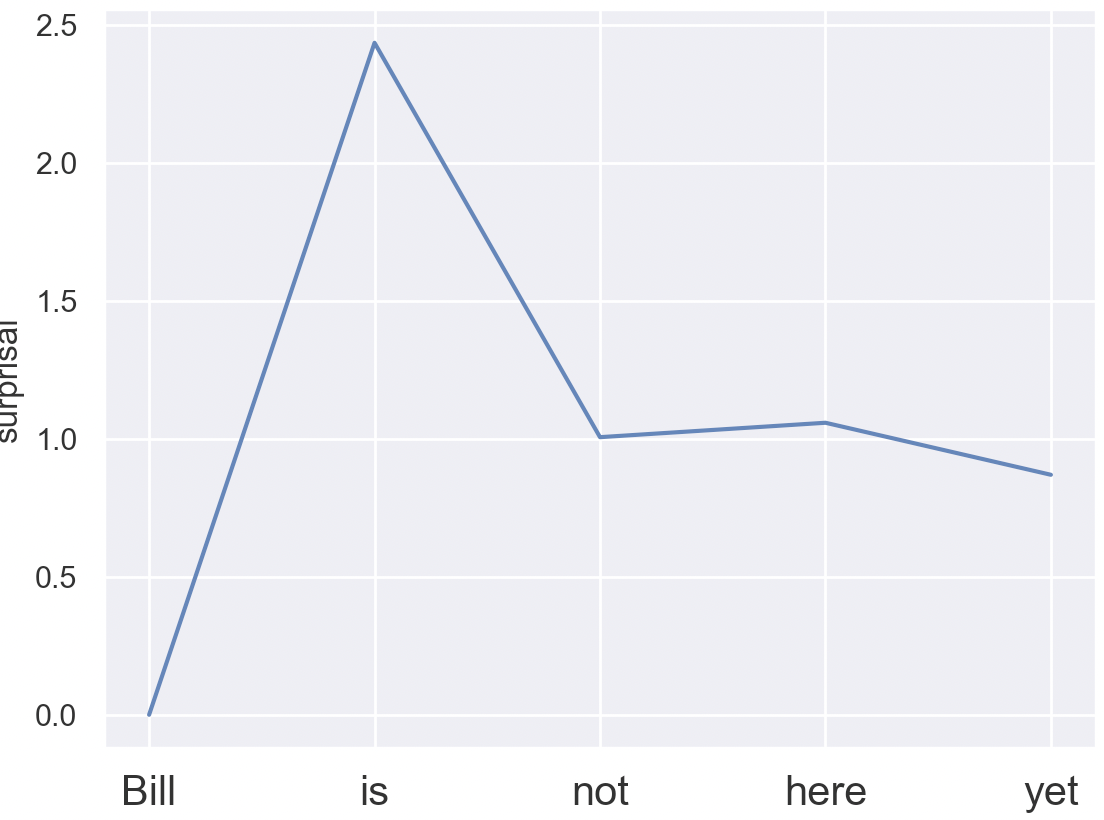
\includegraphics[width=.42\linewidth]{good1} }}
    \subfloat[Ungrammatical]{{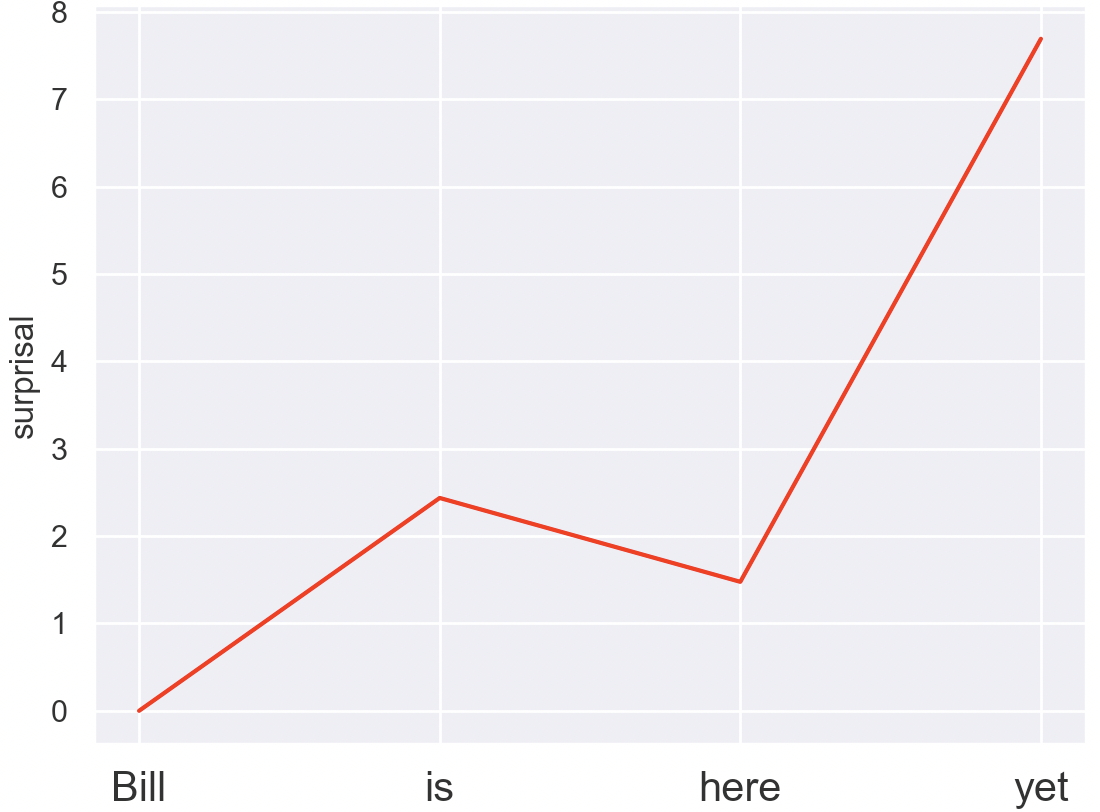
\includegraphics[width=.42\linewidth]{bad1} }}
    \qquad
    \subfloat[Grammatical]{{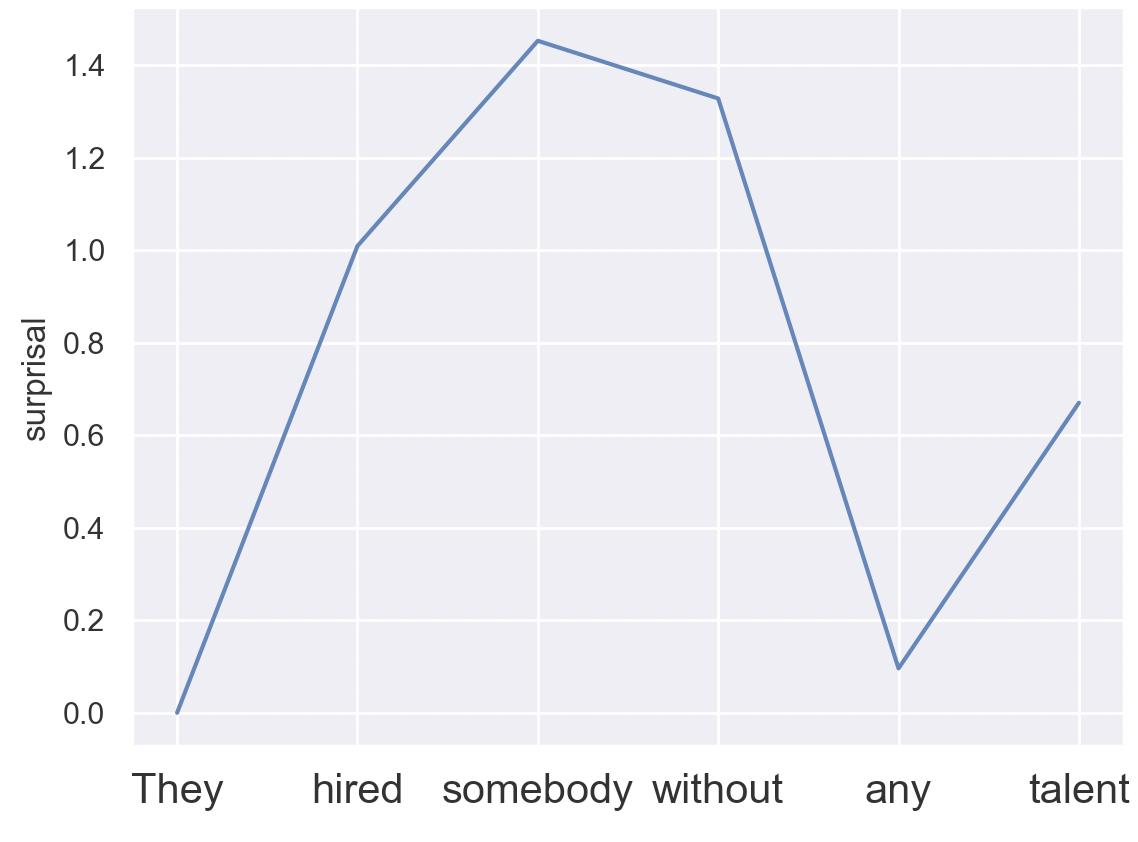
\includegraphics[width=.42\linewidth]{good2} }}
    \subfloat[Ungrammatical]{{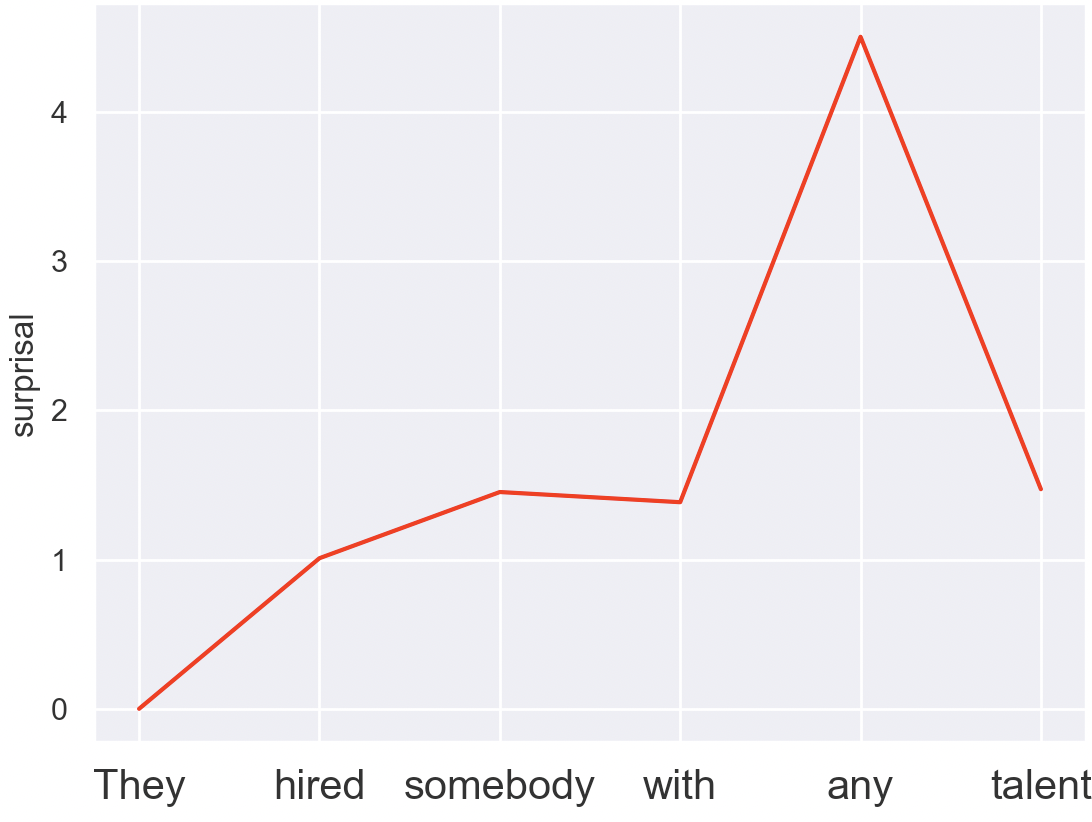
\includegraphics[width=.42\linewidth]{bad2} }}
    \caption{}
    \label{fig:example}
\end{figure}

\subsection{Robustness of Negative Polarity Items to Intervening Material}
Syntactic dependencies are unchanged by the presence intervening material. In the following example, the presence of a negative polarity item (anymore) is due to syntactic licensing by negation (don't); modifying the object doesn't change the sentence structure, so it has no effect on NPI licensing:
\begin{exe}
\ex
\begin{xlist}
\ex We don't go to the supermarket anymore.
\ex We don't go down the block to the supermarket that is owned by Mark anymore. 
\end{xlist}
\end{exe}
We showed in the previous subsection that LSTMs have expectations for negative polarity items, so we attempt to determine whether those expectations remain over intervening material. For this subsection, we designed 10 sentences base sentences with NPI items. Each of the base sentences comes in three varieties: minimal intervening material (enough to make the sentence grammatical), 3-5 words of additional intervening material, and 6-10 additional words between the negative licensor and the polarity item. In all cases the intervening words modify the object of the base sentence.
\subsection{Ability to License Multiple Negative Polarity Items}
In most cases, a negative context can license multiple negative polarity items.
\begin{exe}
\ex
\begin{xlist}
\ex He didn't want to go with anybody anywhere
\ex [*]{He did want to go with anybody anywhere} 
\end{xlist}
\end{exe}

\subsection{Licensing of Negative Polarity Items Between Clauses}
Just because one section of a sentence is in a negative context does not mean that it is appropriate to use a negative polarity item in another clause. In the following example, the dependent clause is fixed as negative and the independent clause (which contains the NPI) is varied, so only the first variation is correct:
\begin{exe}
\ex
\begin{xlist}
\ex Because he was not tired, he was not even sleeping
\ex [*]{Because he was not tired, he was even sleeping} 
\end{xlist}
\end{exe}
In this subsection we attempt to determine whether LSTMs are capable of understanding syntactic structure with regards to negative polarity items. In order to do this we designed 10 base sentences. Each sentence begins with a negative clause, and the grammatically correct version has a second negative clause and NPI wheras the incorrect version has a second postive clause and NPI.
\section{Document Body}


\end{document}
